\documentclass[border=3pt]{standalone}
\usepackage{tikz}
\usetikzlibrary{arrows.meta,calc,positioning}
\tikzset{pin/.style={-{Stealth[length=5pt]}},
  blk/.style={draw, thick, minimum width=14mm, minimum height=16mm, font=\sffamily\small}}
\begin{document}
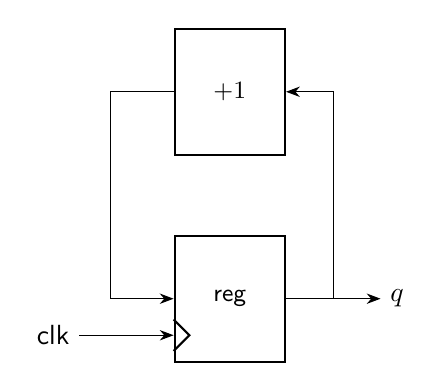
\begin{tikzpicture}[font=\sffamily, node distance=12mm]
  \node[blk] (reg) {reg};
  \draw[thick] ($(reg.south west)+(0,1.5mm)$) -- ++(2mm,2mm) -- ++(-2mm,2mm);
  \node[blk, above=10mm of reg] (add) {$+1$};
  % output q, tapped up into the incrementer
  \draw[pin] (reg.east) -- ++(12mm,0) node[right]{$q$};
  \coordinate (tap) at ($(reg.east)+(6mm,0)$);
  \draw[pin] (tap) |- (add.east);
  % incrementer output back into d
  \draw[pin] (add.west) -- ++(-8mm,0) |- (reg.west);
  % clk straight in from the left at the wedge
  \draw[pin] ($(reg.south west)+(-12mm,3.5mm)$) node[left]{clk} -- ($(reg.south west)+(0,3.5mm)$);
\end{tikzpicture}
\end{document}
